\subsubsection{Den statiske side af design}
\begin{figure}[h]
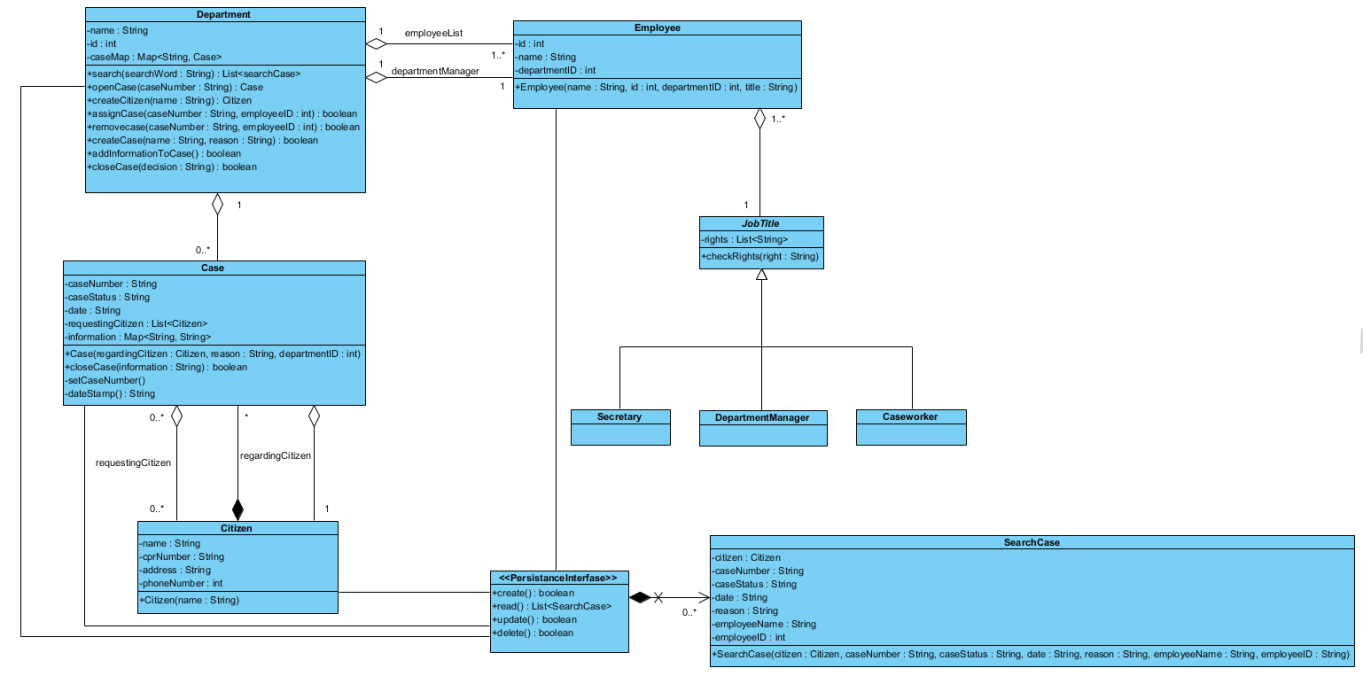
\includegraphics[width = \linewidth]{./PNG/design/fulddesignklassediagram.PNG}
\caption{Klassediagrammfuld. For fuld størrelse se interne bilag afsnit \ref{sec:diverse} figur \ref{fig:fuldDesignKlasseDiagram}}
\label{fig:desginklasse}
\end{figure}
Diagrammet i \ref{fig:desginklasse} beskriver de klasser vi har fundet, der skal implementeres i systemet. Hver klasse har attributter og en del skal have skrevet getter / setter-metoder, men for at diagrammet ikke skal blive for stort og uoverskueligt, valgte gruppen at undlade dem.\\
Diagrammet er blevet designet med tanker på en tydelig lagdeling og repræsentere systemets domænelag. Det blev besluttet at ”Department”-klassen skulle benyttes som facadeklasse til præsenta- tionslaget, mens datahandler interfacet bruges til kommunikation mellem domæne- og persistentslag.\\
\textbf{Department – Facade klasse}\\
Der var særligt fokus på attributterne: ”id” af typen int og ”caseMap” af typen Map\textless String, Case\textgreater . Det var tænkt at ID skulle bruges til at godkende adgangen til sager i databasen, for at imødekomme projektets ”Dataafgrænsning”. ID er af typen int, for at holde den simpel. Kravet til dataafgrænsningen er, at en ansat der henter information omhandlende en borger, ikke må blive gjort opmærksom på sager, der administreres af andre afdelinger end ansattes egen.\\
Tanken bag attributten ”caseMap”, var at department skulle have en liste af case-objekter som kunne bruges til at hente de relevante informationer frem for at sende dem til præsentationslaget. Der blev valgt at bruge et Map da Key/Value-strukturen gør det nemmere at finde en sag. Den Key der blev valgt til caseMap er caseNumber og skal bruges til metoden openCase(…).\\
Klassens metoder, som ”search(…)”, ”openCase(…)”, mm. er designet til at håndtere den logik, som controllerne fra præsentationslaget skal bruge. Metoderne repræsentere de funktioner som er ønsket i det grafiske userinterface (GUI).\\
Når metoden ”search(…)” kaldes, skal logikken først hente data fra persistenslaget. Dette sker gennem Interfacet PersistanceInterface som opretter et objekt af klassen ”SearchCase”, som er designet til at være en dataklasse i domænelaget, for data der er relevant til en brugers søgeord.\\ \\
\textbf{SearchCase – Dataklasse}\\
Klassen består af en constructor med attributterne: ”citizen”, ”caseNumber”, ”caseStatus”, ”date”, ”reason”, ”employeeName” og ”employeeID”. Disse informationer er ikke et udtryk for alt der ligger i en sag, men er nok til at præsentere en borgers sag. \\
Hvis der er et ønske om at hente den fulde sag, gøres dette ud fra ”caseNumber”-attributten gennem ”openCase(…)” metoden, fra ”Department”-klassen. Den data der er relateret til en sag, hentes fra persistenslaget, gennem interfacet ”PersistanceInterface”.\\
\\
\textbf{PersistanceInterface – Datahandler interface}\\
For at behandle dataflowet mellem persistenslaget og domænelaget, er der blevet designet et interface med metoderne: ”create()”, ”read()”, ”update()” og ”delete()”. Disse metoder blev valgt for at kunne oprette, hente, ændre og slette data, som opbevares i persistenslaget. For at domænelaget kan sende dataforespørgsler til persistenslaget, skal der implementeres klasser med det påkrævede interface i persistenslaget.\\ 
\\
\textbf{Case : Employee : Citizen – Objektklasser}\\
Objektklasserne blev designet med tanken om at præsentationslaget og persistenslaget, skulle arbejde med konkrete instanser af disse. Persistenslaget skulle tilføje den data, som var forbundet med objektet, som blev kaldt gennem domænelaget. Præsentationslaget skulle registrere indholdet i objekterne, pakke det ud og præsentere det som ønsket. \\
\\
\textbf{JobTitle – Rollebaseret kontrol}\\
Superklassen ”JobTitle” blev designet til at kontrollere en given medarbejders rettigheder i systemet. Der blev taget udgangspunkt i tre jobstillinger, som blev skrevet op som subklasser - sekretær, sagsbehandler og afdelingsleder. Når en medarbejderklasse blev oprettet, skulle det være et krav, at de fik tildelt en stilling (JobTitle). Denne stilling skulle kunne ændre sig i systemet, f.eks. på grund af en forfremmelse, uden at medarbejderen skulle registreres på ny i systemet.\\
Stillingen som en medarbejder blev tildelet, skulle begrænse funktionaliterne medarbejder har adgang til. 
Dette sikrede de kun havde adgang til de områder, som var nødvendig til at udfører deres opgave. 
En sekretær skulle f.eks. ikke kunne andet end at registrere en person, som søger behandling samt årsagen for at der søges. En sagsbehandler skulle have fuld adgang til relevante sager, dvs. kun sager der er oprettet i den afdeling sagsbehandler er tilknyttet. En afdelingsleder skulle kunne det samme som en sagsbehandler, men også kunne styre hvilke sager de forskellige sagsbehandlere skulle arbejde på.\\
 \\ \\ \\ \\
\textbf{Multiplicitet/Multiplicity – Klassernes forbindelser}\\
Forbindelserne mellem klasserne i designdiagrammet, består primært af aggregeringer. Klassen ”Employee” er forbundet med en many-to-one aggregering til klassen ”JobTitle”. Dette er blevet valgt, da objekter af klassen ”JobTitle” ikke skal blive slettet, hvis et ”Employee”-objekt fjernes. Tanken der ligger til grund for dette, er at ”JobTitle” kan være forbundet til flere forskellige ”Employee”-objekter. \\
Klassen ”Department” er forbundet til ”Employee” med to aggregeringer. Første aggregering er ”employeeList”, som er en one-to-many relation. Aggregeringen er blevet lavet, for at indikere at der kan være mange der arbejder i samme afdeling, men det skal stadig være muligt at slette en ”Department”, uden at slette ”Employee”-instanserne. Anden aggregering er ”departmentManager”, som er en one-to-one relation. Denne aggregering er blevet lavet, for at demonstrere at der altid skal være en leder i en afdeling. Igen skal det være muligt at slette en ”Department”, uden at det sletter ”Employee”.\\
Klassen ”Department” er forbundet til ”Case” med en enkelt aggregering. Dette er en one-to-zero-or-more forbindelse, som betyder at en afdeling ikke altid har nogen sager, men en sag er altid forbundet til en afdeling. Aggregeringen blev valgt, da en sag ikke forsvinder, hvis afdelingen bliver fjernet. \\
Klassen ”Case” er forbundet med to aggregeringer til klassen ”Citizen”, som også er forbundet med en komposition tilbage igen. Den første aggregering der er lavet, er en zero-or-many-to-zero-or-many relation, som omhandler en sags henvisning. En person kan blive henvist af nul eller flere personer, omhandlende det samme problem og på samme måde er det også muligt for en person at have henvendt sig for at få oprettet nul eller flere sager. Anden aggregering er lavet af samme grund som kompositionen er. En ”Citizen” kan have en til flere sager i gang på en gang, men en sag skal altid være angående en enkelt ”Citizen”. Aggregeringen er anvendt da det skal være muligt at fjerne en ”Case” fra systemet, uden at fjerne den ”Citizen” sagen omhandler. Kompositionen er derimod blevet brugt, da en ”Case” altid vedrører en ”Citizen”, og hvis denne fjernes fra systemet, skal de relaterede ”Case”-objekter fjernes, da de ikke længere vedrører nogen.\\
Klassen ”SearchCase” er forbundet med en komposition fra interfacet ”PersistanceInterface”. Da et interface ikke kan instantieres, har det ikke nogen multiplicitet. Kompositionen er blevet valgt, da ”SearchCase” ikke fungere uden interfacet, og forsvinder derfor, hvis interfacet fjernes.